\documentclass{article}

% Enables shell escape for LuaLaTeX
\usepackage{shellesc}

% Font
\usepackage{mlmodern}

% Margins
\usepackage[margin=1in]{geometry}

% Math symbols, proof environments
\usepackage{amsmath, amsthm, amssymb}

% Use this package for matrices
\usepackage{array}

% Images and positioning
\usepackage{graphicx, float, tikz}

% Trees
\usepackage{forest}

% Plots
\usepackage{pgfplots}

\usepackage{xcolor}

\usepackage{parskip}
\usepackage[T1]{fontenc}

% Tables
\usepackage{multirow}

% My definitions
\usepackage{mathdefs}
\usepackage{quantumdefs}

\title{Eigensolver Report}

\author{Jason Cheng}

\date{\today}

\begin{document}

\maketitle

\section*{Implementation}

My implementation closely follows the ideas in the lecture notes/the paper
(Cerezo 2022). The important functions are
\begin{itemize}
  \item
  \verb|ansatz| --- Implements \( V(\theta) \) as described in the paper

  \item
  \verb|cost| --- Calculates the cost function according to the formula in the
  lecture notes

  \item
  \verb|grad| --- Calculates the cost function gradient according to the formula
  in the paper

  \item
  \verb|read_ansatz| --- Reads the eigenvectors from \( V(\theta) \)

  \item
  \verb|train| --- Implements gradient descent optimization

  \item
  \verb|train_incremental| --- Train layers incrementally rather than all together
\end{itemize}

\verb|cost| and \verb|read_ansatz| both use experimental results to estimate the
vectors being read. Since it's based on probability, that means the eigenvectors
produced by \verb|read_ansatz| are missing their signs.

\verb|train_incremental| is an experimental training approach. It repeatedly
adds new layers and optimizes only the new layers, holding the parameters for
the old layers constant. This improved efficiency, but at the cost of some
accuracy.

For gradient descent, I used PyTorch's \verb|SGD| optimizer, which is gradient
descent with momentum. I hoped that the momentum would help prevent getting
stuck in local minimums.

\section*{Experiments}

I evaluated my results based on two metrics: cosine similarity between the
measured eigenvectors and the true eigenvectors (obtained with
\verb|np.linalg.eig|), and the magnitude of the gradient. This helps determine
the cause of bad performance. For example, if gradient magnitude converges while
similarity fails to converge, we could be stuck in a local minimum. 

\subsection*{Hyperparameters}

\renewcommand{\arraystretch}{1.5}
\begin{tabular}{|l|l|l|l|l|l|}
  \hline
  ID & Qubits & Layers & Iterations & Learning rate & Similarity \\
  \hline
  1 & 2 & 2 & 100 & 0.01 & 0.9997 \\
  \hline
  2 & 3 & 6 & 150 & 0.001 & 0.9986 \\
  \hline
  3 & 3 & 4 & 200 & 0.001 & 0.9338 \\
  \hline
  4 & 3 & 4 + 2 & 100 + 100 & 0.001 & 0.9834 \\
  \hline
  5 & 4 & 16 & 200 & \( 10^{-4} \) & 0.9732 \\
  \hline
  6 & 4 & 4 & 1000 & \( 10^{-5} \) & 0.9322 \\
  \hline
  7 & 4 & 8 & 1300 & \( 10^{-6} \) & 0.8239 \\
  \hline
  8 & 4 & 4 + 4 + 4 + 4 & 200 + 200 + 200 + 200 & \( 10^{-4} \) + \( 10^{-4} \) + \( 10^{-5} \) + \( 10^{-5} \) & 0.9247 \\
  \hline
\end{tabular}

TBD: hasn't finished running

\section*{Discussion of results}

Experiment 3 shows what happens when we decrease the number of layers. In the
paper, they only used 3 layers for up to 10 qubits, so I wondered if I could
replicate the same results using fewer layers. It turns out having fewer layers
decreases accuracy. Here are the training graphs of experiment 2 and 3:

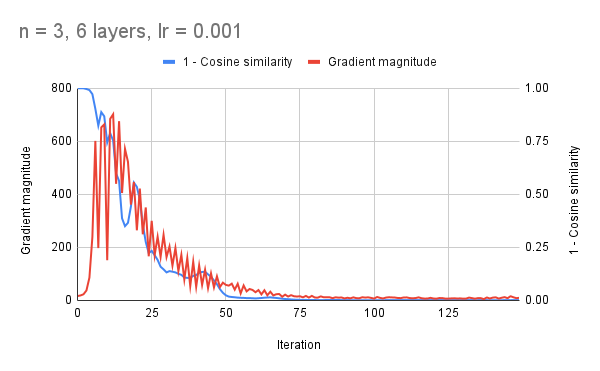
\includegraphics[width=0.8\linewidth]{img/n3l6r3.png}

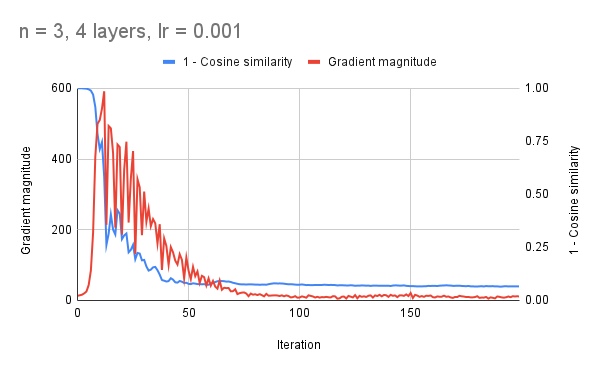
\includegraphics[width=0.8\linewidth]{img/n3l4r3.png}

We can see that the gradient converges to around the same value, but the
similarity fails to converge. This might be because there are fewer parameters,
so each parameter is more affected by the gradient. Thus, a smaller learning
rate might fix the problem. In experiment 6, I tested this theory by decreasing
the learning rate by a factor of 0.1 compared to experiment 5, but I still had a
lower accuracy. In experiment 6, I tried to decrease the learning rate even
further but was not able to finish training because it took so long. The
similarity was still increasing slightly when I stopped the simulation.

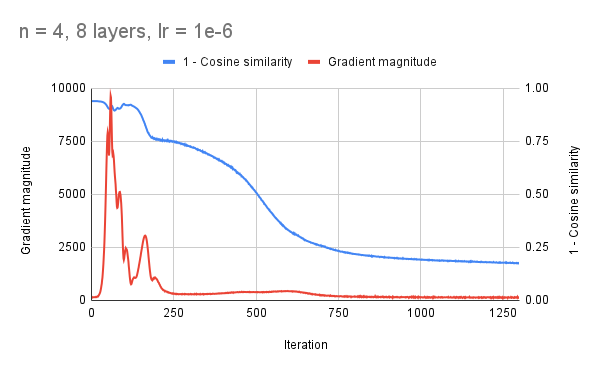
\includegraphics[width=0.8\linewidth]{img/n4l8r6.png}

Experiment 8 shows the effect of my incremental training approach:

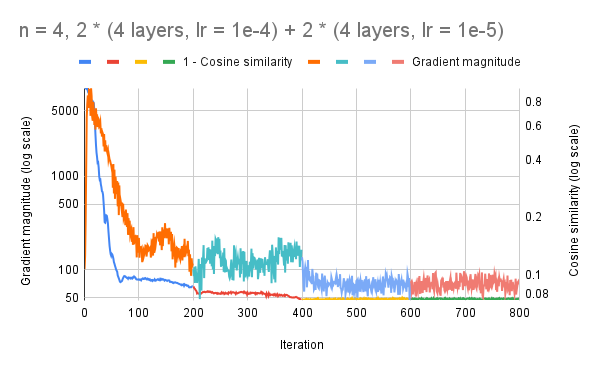
\includegraphics[width=0.8\linewidth]{img/n4l4l4r4l4l4r5.png}

Each color represents a set of 4 layers. The first two sets were trained with
learning rate \( 10^{-4} \) and the second two sets were trained with learning
rate \( 10^{-5} \). The accuracy isn't as good as experiment 5, where I trained
all 16 layers together. However, it was much more efficient because I was only
training \( 1 / 4 \) of the parameters at once. Experiment 5 took 2 days to
train, while experiment 8 finished in a few hours.

\end{document}
